\documentclass{UoYCSproject}
\graphicspath{ {./figures/} }

%\addbibresource{dummyBib.bib}
\author{Katie Maison}
\title{Agile ticket estimation with BERT}
\date{2024}
\supervisor{Peter Nightingale}
\BSc

\dedication{To my son}

\acknowledgements{
    I would like to thank my goldfish for all the help it gave me
    writing this docume

    As usual, my boss was an inspiring source of sagacious advice.
}

% Document

\begin{document}
    \pagenumbering{roman}
\setcounter{page}{1}

\maketitle
\listoffigures
\listoftables
%\renewcommand*{\lstlistlistingname}{List of Listings}
%\lstlistoflistings

\chapter{Introduction}
\label{ch:introduction}
\setcounter{page}{1}
\pagenumbering{arabic}

Introduction
Late delivery of software projects remains an ever present challenge, often attributed to the inherent uncertainties and complexities associated with development.
There are multiple factors that affect the delivery of a software project, however it is clear that project planning plays a role in this [45]. \par
Agile Software development is a type of iterative planning method where a project is broken up into smaller “user stories” or tickets, each defining a specific task or part of a project that must be completed.
Generally each ticket has an estimate attached to it, defining the time or effort it will take to finish.
Some projects use time-based estimates like hours or days to estimate tickets, others teams assign “Story Points”, an abstract unit of perceived complexity, risk, and effort involved in implementing a specific feature or piece of functionality [Book].
For example, a Story Point value of 1, may be equated to 2 hours work or less, 8 around 22 hours of active work on a ticket or 11 hours for 2 people.
It is common for the Story Point scale used to be an adjusted fibbonaci, of 1, 2, 3, 5, 8, 13, 15, 20, 40, 100.
Estimates enable a Team leader to plan what tickets can be completed in a “sprint”, or “iteration”, usually a period of 2-4 weeks, based on how many points they think the team will be able to do [Agile planning and development methods].
The process for estimating tickets can be time consuming, the faster that a ticket is estimated, the faster it can be planned for completion.
Furthermore, the more accurate an estimation is, the more likely it is that a release, which in agile, is a collection of tickets associated with features or bug-fixes in a release, can be delivered on time, as the work will have been planned accordingly. \par

When a ticket is created, it is placed into a to-do list of tickets called a “backlog”.
Tickets in the backlog are then estimated for their effort or time to complete, and are then ordered according to multiple factors including this estimate and the priority of the ticket.
Generally in projects, work cannot be carried out on a ticket until it has been estimated.
This emphasises the importance of both the speed and accuracy of ticket estimation in the successful management of projects.
Automated ticket estimation may enable the correct prioritisation of tickets before any estimation activities are carried out by the team or members of the team.
By using a large language model, the information provided in a tickets title and description can be used as features in a classification neural network.
The model proposed in this paper is intended to participate in the estimation process rather than perform the estimation as the source of truth.
This is because incorrect estimates can have severe consequences on project planning, a model would need to be extremely accurate in order to be trusted to estimate the ticket correctly.
In practice the model participation can happen in multiple ways.
The model may act as an advisor for the “expert” who is estimating tickets.
Alternatively the model may participate in agile poker sessions with members of a project, whereby engineers play a “game” where everyone chooses a card that equates to the value that they want to estimate, then discuss and re-estimate until a consensus is reached [15]. \par

In order to simplify the problem, the model proposed in this paper will be able to classify tickets into 3 categories, “Small”, “Medium” and “Large”, whereby a ticket is classified as “Small” if it is estimated to take less than 2 days, “Medium” if it is estimated to take between 0 and 3 hours, medium if its 3-8 hours, and “Large” if it is estimated to take more than 8 hours.
When inspecting data from a project in a large automotive company, who estimate using minutes and hours, it was found that the accuracy of ticket estimation was 72\% when usimg the above categories.
Furthermore, I am aiming to ensure that the model takes less than 4 hours to train, and less than 1 second to classify a ticket once trained.
This is so that the model can be used in real time, and can be retrained on a regular basis to ensure that it is up to date with the latest data, ensuring continuous learning but also reduce costs. \par

\chapter{Literature Review}
\label{ch:literature-review}
This section discusses the current research into methods of ticket estimation, including with Deep learning, as well as in the broader field of Natural Language Processing.
It summarises and analyses existing work as well as highlighting unknowns within the topics.

It is broken down into 3 sub-sections.
First “Estimation in Software Engineering Projects” focuses on research about effort and time estimation as a concept, as well as research into techniques for doing estimations.
The next sub-section focuses on relevant research into Large Language Models and Natural Language Processing.
Lastly, the “Agile Estimation with Deep Learning” looks at Deep learning models specifically for classification of text, particularly of Agile Tickets for estimation.

\section[Effort Estimation]{Effort Estimation}
\label{sec:effort-estimation}
Current research into estimation in agile projects mostly centres around how estimations are produced and what scale they use.
There are many methods for estimating tickets or projects that have been examined in academic research.
They can be sorted into two main categories, Judgement-based approaches and Model-based approaches (discussed below) [37].
\subsection{Judgement-based approaches}
\label{subsec:judgement-based-approaches}

Judgement-based approaches rely on the knowledge of experts about the field or project in question, who can make an estimate based on their experiences and knowledge on how much effort a ticket will take to complete.
The simplest judgement based approach, expert judgement, is a single expert estimating the ticket by themselves, however group estimation techniques such as Planning poker, whereby team members play a “game” to reach an agreement on the Story Point estimate of a tickets are also popular.
Research has been done to examine the accuracy of these techniques by looking at the result of the same ticket estimated with both, showing that planning poker is more accurate that individual expert estimates [38, 39]. Other
A survey was performed in 2015 to determine the state of the practice of Effort Estimation of Agile Software Development.
The research surveyed 60 users of agile practices across 16 different countries. It established that 63\% of participants use Planning poker to perform estimations followed by 47\% used analogy (whereby parallels are drawn from previous stories and they are used to decide an estimate for new stories [source for this]) and expert judgment (38\%)[48].

\subsection{Model-based approaches}
\label{subsec:model-based-approaches}
Model Based Effort Estimation
In the last 30 years, many Algorithmic-Based Approaches have been proposed to automate the estimation of tickets
and projects.
In 1981, the Constructive Cost Estimation Model ($COCOMO$) model was proposed by DR. Berry Boehm [41].
The basic $COCOMO$ model defines the effort required to complete a project to be $a^2 \times (KLOC)a^2pm$.
Where $KLOC$ is kilo lines of code, $a$ is a constant depending on the type of project and is expressed in person months ($pm$), the detailed version adds effort multipliers for each phase of a project, splits the effort estimation into subsystems and adds various extra multipliers to improve accuracy.
Although this model can achieve a mean average accuracy of 91\% for effort estimation on projects (need to check the validity of this, check for another source, this seems very high) [43], the model requires a lot of input information, including Lines of Code, number of files, number of external interfaces and developer experience with the technical stack.
COCOMO, as well as other model based estimators like SLIM[51] and regression models are used much less in agile software development than previously in non-agile development methods [48, 40] due to the estimations being for tickets rather than for entire projects, where the attributes needed are more readily available and relevant.
As in a ticket rather than in a project, the main information is the textual description, with the shift towards agile software development, focus has shifted towards researching how we can leverage Natural Language Processing in order to estimate story points.

\section{Large Language Models}
\label{sec:large-language-models}
Large Language Models (LLM) are a type of artificial intelligence model that is designed to understand, generate
or manipulate human language.
These models are characterized by their size and complexity, often consisting of millions or even billions of parameters.
Large language models are built on advanced deep learning architectures and are typically pre-trained on massive amounts of textual data (corpus) before being fine-tuned for specific tasks. \par

In 2017, transformer based architecture was introduced in a model proposed by Vaswani et al [Transformer].
It has become the foundational model for a variety of natural language processing (NLP) tasks, including text classification, question answering, summarization, and translation.
The transformer based architecture is a type of neural network architecture that is designed to process sequential data, such as text, and is based on the concept of attention.
The core innovation of this architecture is the introduction of 'self-attention'.
Self-attention allows a model to weigh the importance of different words in a sequence when processing each word, rather than relying on a fixed-length context window, like in recurrent neural networks (RNNs).
This means that a model can capture long-range dependencies effectively.
The self-attention mechanism also allows the model to process all words in a sequence simultaneously, rather than sequentially, therefore improving the training speed as it allows parallelization.
\par
In June 2018, Generative Pre-Trained Transformers (GPT) was introduced by OpenAI in the paper "Improving Language Understanding by Generative Pre-Training".
GPT follows an autoregressive approach during both pre-training and fine-tuning, this means that the model generates text sequentially, predicting the next word in a sequence based on the preceding context.
This allows GPT to capture complex dependencies and relationships in language, however GPT only looks at the context of previous words, left-to-right rather than bidirectionally like later models.

In October 2018, the Bidirectional Encoder Representations from Transformers (BERT) model was introduced by Devlin et al.
[BERT].
BERT is a large language model that uses the transformer architecture and is pre-trained on a large corpus of unlabelled text, including the entire Wikipedia corpus and a large book corpus, totaling 3,300M words.
It is trained using a masked language model (MLM) objective, where random tokens in a sequence are masked, and the model is trained to predict those masked tokens.
BERT is considered a landmark in the development of large language models, for multiple reasons.
An important difference between BERT and previous language models is that it is bidirectional, meaning that it can
use the context of both the left and right side of a word when processing it, enabling the model to capture richer contextual information compared to previous unidirectional models.
At time of release, BERT outperformed all other Large Language Models on the General Language Understanding Evaluation (GLUE Benchmark), a set of tasks that are designed to measure the performance of models that aim to understand language.
An average of 79.6\% on the $GLUE$ benchmark tasks was achieved by the $BERT_{base}$, 4.4\% higher than the previous highest score achieved by OpenAI's GPT.

The release of BERT and GPT in 2018 was followed by the proposal of many new models based on the transformer architecture in 2019.
XLNet was introduced by researchers at Google and Carnegie Mellon University, it is another transformer-based language model that extends the bidirectional context understanding of BERT while addressing some of its limitations.
XLNet uses a permutation language model (PLM) objective.
Instead of masking random tokens, XLNet considers all tokens in the sequence as potential candidates for prediction.
This means that the model is trained to predict the probability distribution over all possible permutations of the sequence.


% This part is maybe not neccessary?
An important part of Large language models is Tokenization, which is the process of splitting a string into a list of
tokens.
A token can be a word, sentence, paragraph or even a single character.
Tokenization is performed by a Tokenizer, which is a class that defines a vocabulary and methods for encoding.
The vocabulary is a list of known tokens, for example words from a dictionary or in a particular corpus.
The Tokenizer can then encode a string by breaking it up into tokens and replacing each token with its corresponding integer value from the vocabulary.
One popular tokenizer is WordPiece, which was introduced in 2016 by Google as the tokenization method for BERT [BERT].
WordPiece is a sub-word tokenizer, meaning that it breaks words down into smaller parts, or sub-words.
WordPiece is effective in handling rare or unseen words because it can represent them as a combination of more common sub-word units.
This property is especially valuable for tokenizing text on a niche topic or with unusual vocabulary. \par

Byte Pair Encoding (BPE) is another popular tokenizer, it was first introduced by Philip Gage in the context of text compression in 1994 [BPE].
It is a simple form of dictionary encoding, which iteratively replaces the most frequent pair of bytes in a sequence with a single, unused byte.
Whilst it was an effective text compression algorithm, it was later recognized for its utility in natural language processing (NLP),
and has since been used in many NLP models, including transformer-based models like GPT.

\section{Ticket classification with deep learning}
\label{sec:estimation-with-deep-learning}

In 2018, Choetkiertikul et al.
introduced a significant contribution to the field of software engineering with their paper titled 'A deep learning model for estimating story points.'.
This research, conducted at the University of Wollongong (Australia), presents a model for estimating the story point estimation of tickets (DEEP-SE) and is the most notable research paper on ticket classification with deep learning.
The model uses long short-term memory and recurrent highway network which are both types of recurrent neural network (RNN) architectures.
It defines the task as a regression problem and achieves a standardized accuracy of 52.66\%
\[SA = (1-\frac{MAE}{MAE_{rguess}}) \times 100\]
where $MAE$ is the Mean Absolute Error and $MAE_{rguess}$ is the MAE of a large number (e.g. 1000 runs) of random guesses. Such that $MAE$, defined as \[ MAE = \frac{1}{N}\sum_{i=1}^{N}|ActualSP_{i} - EstimatedSP_{i}|\] where $N$ is the number of issues used for evaluating the performance (i.e. test set), $ActualSP_i$ is the actual story point, and $EstimatedSP_i$ is the estimated story point, for the issue $i$.
The dataset used for this model was 23,313 tickets story points, collected from 16 large open source projects.
This dataset has since been used by other researchers including Phan et al\. who looked at the potential and possible challenges of Graph Neural Network text
classification in story point estimation [5].
Their proposed model achieved an accuracy as high as 80\% on some projects within the dataset when classifying tickets into 6 'buckets' of story points.

However, it is clear that there is a research gap into ticket effort estimation using large language models such as BERT.


\chapter{Problem Analysis}
\label{ch:problem-settings}


\chapter{Methodoloy}
\label{ch:methodology}
This section introduces the proposed model for the classification of tickets.
It covers explanation of the datasets, preprocessing, data augmentation methods and the architecture of different models that were evaluated as well as justification of the final model.
The last subsection discusses the ethics of the problem.

\section{Datasets}\label{sec:datasets}
The datasets used to evaluate this model come from a large automotive software company, containing a total of 40,000 tickets, across 12 projects.
Every ticket has a title, or a "Summary" that is a short description of the ticket, usually less than X characters.
It then has a description, this a longer piece of text that explains what the aim of the ticket is. \par

\begin{figure}[h]
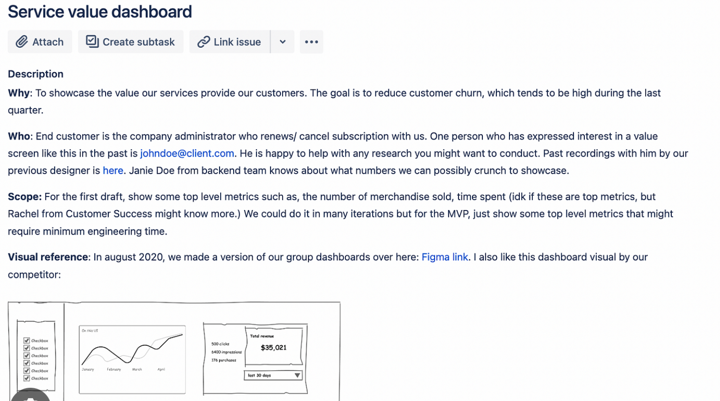
\includegraphics[width=\textwidth]{ticket-example}
\caption{an example ticket}
\label{fig:figure}
\end{figure}

For the dataset in question, the word count is between 2 and 1000, as shown in figure 3.2.

% word count figure %

The dataset has two types of tickets, ones that have been estimated with a specific time and ones that have been estimated with story points.
Ones that have been estimated with a specific time also have the "Actual time spent" logged on them.
This is useful as it may help our model become more 'intelligent' than a person estimating them as we can use ground truth values. \par


% Visualisations/table of the dataset %


\section{Pre-Processing}\label{sec:preprocessing}

    The main features of each ticket is its summary and description.
The description is written with Jira Markdown syntax, for example it allows formatted blocks of code to be added with the syntax {code:java} {code} and h[1-6]. formats the text following as a heading.
In order to remove this syntax and reformat the text as plain text, a set of regex replace rules were used.
These rules removed blocks of code and formatting syntax, but also has anonymised the data by removing mentions of users, for example @KatieMaison which stops the model learning to differentiate the estimation for the ticket by a user as a feature, as this may have ethical considerations. \par

The text string used as an input to the model is the summary prepended to the description.
This is because usually in a ticket, a title has the most important information in it, often containing keywords about the contents of the ticket. \par

In order to enable classification, an additional column $class$ was added to the dataset, where $class(ticket) \in \{0,1,2\}$, where 0 is small, 1 is medium and 2 is large.
"Small" tickets have been defined as those that take less than 1 hour to complete and are estimated to be 0-1 Story Point in effort.
"Medium" tickets have been defined as those that take between 1 and 5 hours, or are estimated to be between 1 and 5 story points.
"Large" tickets are defined to take more than 5 hours to complete, or have more than 5 story points as an estimate.
% How the dataset was split up %
    \item "Small": if $storypoint(ticket) \in \{0,1\}$ or completion time $< 1$ hour.
  \item "Medium": if $1 \leq storypoint(ticket) \leq 5$ or $1 \leq$ completion time $\leq 5$.
  \item "Large": if $storypoint(ticket) > 5$ or completion time $> 5$ hours.

%\begin{tabular}{|p{7cm}|p{2cm}|p{1.5cm}|p{1cm}|}
%  \hline
%  Ticket Description & Story Point Estimate & Time Logged & Class\\
%  \hline
%  As part of the AUTOSAR project, we need to implement the Controller Area Network (CAN) communication module. This module will facilitate communication between various electronic control units (ECUs) within the vehicle.
% & 5 & N/A & 1 \\
%    \hline
%
%  Row 2, Col 1 & Row 2, Col 2 & Row 2, Col 3 & c2 \\
%  \hline
%\end{tabular}

\section{Data Augmentation}\label{sec:data-augmentation}
In order to increase the generalisation of the model and therefore increase accuracy on unseen data, I have opted to use data augmentation to increase the number of data points and also to reduce the class imbalance in the data.
Back translation was tested as an augmentation technique, which is where a ticket is translated into a different language, and then translated back. I used the NLPAug Python library, which allows you to choose a translation model from huggingface to use to translate the text.
However upon inspecting the tickets, there was very little change in the wording of the ticket, and the model over-fit much more quickly, reaching a very small loss and test accuracy stagnated.
Instead, paraphrasing had better results.
To do so, I used a pretrained model from the huggingface library, "Finetuned GhatGPT paraphraser on T5-base". [paraphraser]
This model is a t5 model, finetuned on a dataset of phrases and their paraphrases.

% Example of paraphrased sentences

I first used the data cleaner described previously to remove the formatting syntax, then ran the paraphraser on every ticket, which took 21 hours on an ATX200 Graphics card.\par

\section{Architectures}\label{sec:architectures}
    The architecture of the model can be described in three parts, Tokenization Layer, Transformer Layers and Classification Head.
    These will be described sequentially in the following sections.\par

\subsection[tokenization-layer]{Tokenization Layer}
    In order to be used in a Large Language Model, textual input needs to be transformed into tokens and embeddings.
    My model uses the BERT Tokenizer, the specific implementation of which is provided by the transformers huggingface library. \par

    \begin{figure}[h]
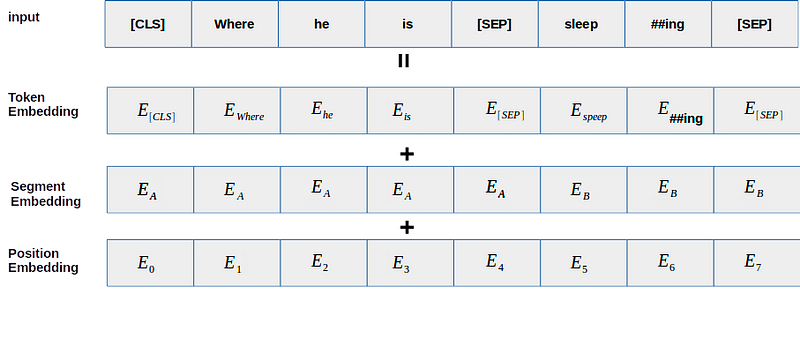
\includegraphics[width=\textwidth]{bert-tokenizer}
\caption{Bert Tokenizer from the Original Bert Paper}
\label{fig:tokenizer-figure}
\end{figure}

    The tokenizer works by splitting each tickets description $T$ into individual tokens, then converting these into a numerical value from the models vocab.


\section{Ethical Considerations}\label{sec:ethical-considerations}

\chapter{Experimental Settings}
\label{ch:experimental-settings}

\chapter{Results}
\label{ch:results}

\chapter{Model as a Service}
\label{ch:model-as-a-service}

\chapter{Conclusion}
\label{ch:conclusion}

\printbibliography

\end{document}
